% Options for packages loaded elsewhere
\PassOptionsToPackage{unicode}{hyperref}
\PassOptionsToPackage{hyphens}{url}
%
\documentclass[
]{book}
\usepackage{amsmath,amssymb}
\usepackage{lmodern}
\usepackage{ifxetex,ifluatex}
\ifnum 0\ifxetex 1\fi\ifluatex 1\fi=0 % if pdftex
  \usepackage[T1]{fontenc}
  \usepackage[utf8]{inputenc}
  \usepackage{textcomp} % provide euro and other symbols
\else % if luatex or xetex
  \usepackage{unicode-math}
  \defaultfontfeatures{Scale=MatchLowercase}
  \defaultfontfeatures[\rmfamily]{Ligatures=TeX,Scale=1}
\fi
% Use upquote if available, for straight quotes in verbatim environments
\IfFileExists{upquote.sty}{\usepackage{upquote}}{}
\IfFileExists{microtype.sty}{% use microtype if available
  \usepackage[]{microtype}
  \UseMicrotypeSet[protrusion]{basicmath} % disable protrusion for tt fonts
}{}
\makeatletter
\@ifundefined{KOMAClassName}{% if non-KOMA class
  \IfFileExists{parskip.sty}{%
    \usepackage{parskip}
  }{% else
    \setlength{\parindent}{0pt}
    \setlength{\parskip}{6pt plus 2pt minus 1pt}}
}{% if KOMA class
  \KOMAoptions{parskip=half}}
\makeatother
\usepackage{xcolor}
\IfFileExists{xurl.sty}{\usepackage{xurl}}{} % add URL line breaks if available
\IfFileExists{bookmark.sty}{\usepackage{bookmark}}{\usepackage{hyperref}}
\hypersetup{
  pdftitle={Méthodes quantitatives},
  pdfauthor={Paul Hobeika},
  hidelinks,
  pdfcreator={LaTeX via pandoc}}
\urlstyle{same} % disable monospaced font for URLs
\usepackage{longtable,booktabs,array}
\usepackage{calc} % for calculating minipage widths
% Correct order of tables after \paragraph or \subparagraph
\usepackage{etoolbox}
\makeatletter
\patchcmd\longtable{\par}{\if@noskipsec\mbox{}\fi\par}{}{}
\makeatother
% Allow footnotes in longtable head/foot
\IfFileExists{footnotehyper.sty}{\usepackage{footnotehyper}}{\usepackage{footnote}}
\makesavenoteenv{longtable}
\usepackage{graphicx}
\makeatletter
\def\maxwidth{\ifdim\Gin@nat@width>\linewidth\linewidth\else\Gin@nat@width\fi}
\def\maxheight{\ifdim\Gin@nat@height>\textheight\textheight\else\Gin@nat@height\fi}
\makeatother
% Scale images if necessary, so that they will not overflow the page
% margins by default, and it is still possible to overwrite the defaults
% using explicit options in \includegraphics[width, height, ...]{}
\setkeys{Gin}{width=\maxwidth,height=\maxheight,keepaspectratio}
% Set default figure placement to htbp
\makeatletter
\def\fps@figure{htbp}
\makeatother
\setlength{\emergencystretch}{3em} % prevent overfull lines
\providecommand{\tightlist}{%
  \setlength{\itemsep}{0pt}\setlength{\parskip}{0pt}}
\setcounter{secnumdepth}{5}
\usepackage{booktabs}
\usepackage{booktabs}
\usepackage{longtable}
\usepackage{array}
\usepackage{multirow}
\usepackage{wrapfig}
\usepackage{float}
\usepackage{colortbl}
\usepackage{pdflscape}
\usepackage{tabu}
\usepackage{threeparttable}
\usepackage{threeparttablex}
\usepackage[normalem]{ulem}
\usepackage{makecell}
\usepackage{xcolor}
\ifluatex
  \usepackage{selnolig}  % disable illegal ligatures
\fi
\usepackage[]{natbib}
\bibliographystyle{plainnat}

\title{Méthodes quantitatives}
\author{Paul Hobeika}
\date{2022-01-28}

\begin{document}
\maketitle

{
\setcounter{tocdepth}{1}
\tableofcontents
}
\hypertarget{section}{%
\chapter*{}\label{section}}
\addcontentsline{toc}{chapter}{}

Cette page accueille les notes de cours de méthodes quantitatives du M1 de Science Po Strasbourg.

\hypertarget{donnuxe9es-et-vocabulaire-de-la-statistique}{%
\chapter{Données et vocabulaire de la statistique}\label{donnuxe9es-et-vocabulaire-de-la-statistique}}

\hypertarget{les-sources-statistiques-en-sociologie}{%
\section{Les sources statistiques en sociologie}\label{les-sources-statistiques-en-sociologie}}

Nous avons évoqué la semaine dernière l'importance de la connaissance des sources statistiques pour la production de savoirs quantitatifs en sciences sociale. Il en existe différents types, qu'il est important de savoir identifier.

\hypertarget{les-enquuxeates-par-questionnaire-produites-par-les-chercheur-es}{%
\subsection{Les enquêtes par questionnaire produites par les chercheur-es}\label{les-enquuxeates-par-questionnaire-produites-par-les-chercheur-es}}

C'est par exemple le cas des données exploitées dans \emph{La distinction} \citep{bourdieu1979} dont nous avons parlé au premier semestre. A partir d'une problématique de départ parfois abstraite (dans le sens pas directement quantifiable), l'élaboration d'un questionnaire a souvent pour objectif de trouver des éléments empiriques concrets qui permettent de rendre opérationnelles certaines notions ou concepts. Par exemple, dans \emph{La distinction}, le questionnaire porte sur les pratiques culturelles et permet d'opérationaliser empiriquement la notion de \emph{capital culturel}.

\begin{quote}
Remarque : si vous souhaitez produire vous-même des données dans le cadre de votre TER et de la validation du cours c'est tout à fait possible, mais nous n'aborderons pas la méthodologie du questionnaire dans ce cours. De bons manuels sont toutefois disponibles, je vous recommande par exemple celui de \citet{bugeja-bloch2021}, chapitres 3 et 4.
\end{quote}

\hypertarget{les-autres-source-de-premiuxe8re-main}{%
\subsection{Les autres source de ``première main''}\label{les-autres-source-de-premiuxe8re-main}}

En réalité, les chercheur-es peuvent effectuer des traitement quantitatifs sur d'autres types de sources que les données issues d'un questionnaire. Pour cette raison, Fanny Bugeja-Bloch et Marie-Paule Couto font une distinction entre les \textbf{technique d'enquête} et les \textbf{technique d'analyse} des données.

\begin{figure}
\centering
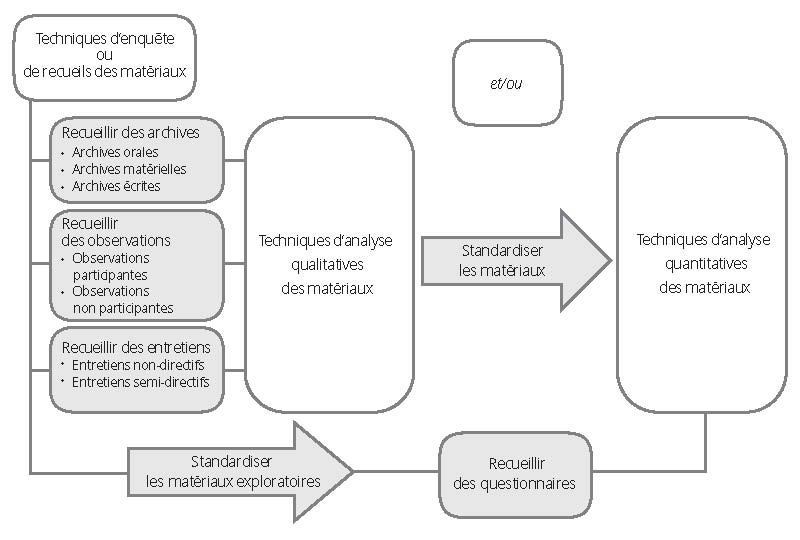
\includegraphics{images/techniquesenquete.jpg}
\caption{Techniques d'enquête et techniques d'analyse \citep{bugeja-bloch2021}}
\end{figure}

Les \textbf{techniques d'enquête} désignent les différents modes de recueil des données : données d'archives, d'entretien ou encore issues d'observation. Les matériaux ainsi produits peuvent ensuite se prêter à différentes formes d'analyse. C'est seulement à ce niveau que l'on peut distinguer méthodes qualitatives et quantitatives. Une analyse qui se fondera sur le commentaire d'un ou quelques extrait d'entretien par exemple sera qualifiée de \emph{qualitative}. Mais ces mêmes matériaux, lorsqu'ils sont \emph{standardisés} et \emph{mis en série} peuvent également être l'objet de techniques d'analyse quantitative. On peut produire des statistiques à partir d'archives \citep{lemercier2008}, à partir d'entretiens (le questionnaire en est un cas particulier) ou encore à partir d'observations \footnote{Un exemple tiré de la sociologie du travail est celui de l'enquête de Jean Peneff sur les urgences. Effectuant une enquête par observation participante en tant que brancardier dans un service d'urgence, il fait un certain nombre de comptages dans l'objectif d'objectiver certaines dimensions du travail aux urgences \citep{peneff1992}.}.

\hypertarget{lanalyse-secondaire-des-donnuxe9es}{%
\subsection{L'analyse secondaire des données}\label{lanalyse-secondaire-des-donnuxe9es}}

Dans de nombreux cas, ce ne sont pas les sociologues ou politistes qui produisent les données qu'ils ou elles exploitent. On parle alors d'\textbf{analyse secondaire des données}. C'est le cas lorsqu'on travaille sur des données de l'Insee ou n'importe quelle base de donnée produite par une administration.

Quelques liens pour accéder aux données de la statistique publique française :

\begin{itemize}
\item
  \href{http://www.progedo-adisp.fr/}{le site de l'Adisp} (Archives de données issues de la statistique publique) , qui rassemble les données de l'Insee et des directions statistiques ministérielles (santé, travail, culture, etc.)
\item
  \href{http://nesstar.ined.fr/webview/}{les données de l'Ined (Institut national de la recherche démographique)}
\end{itemize}

\hypertarget{donnuxe9es-denquuxeate-et-donnuxe9es-de-gestion}{%
\subsection{Données d'enquête et données de gestion}\label{donnuxe9es-denquuxeate-et-donnuxe9es-de-gestion}}

Parmi l'ensemble des données accessibles produites par la statistique publique, on distingue en général deux grandes catégories \citep{desrosières2005} . D'un côté les bases de données produites via une \textbf{enquête par questionnaire} comme évoqué plus haut : elles sont réalisées à partir d'un échantillonage au sein d'une population plus large (voir plus loin pour des définitions de ces termes), et comportent un grand nombre de variables, qui correspondent en général à des questions qui sont posées directement par des enquêteurs ou enquêtrices. De l'autre côté, certaines bases de données sont le \textbf{résultat du travail de gestion de certaines administrations} : par exemple, les employeurs effectuent chaque année ce qu'on appelle une ``déclaration annuelle de données sociales'', dans laquelle ils renseignent une série d'informations sur leurs différents salarié·es (parmi lesquelles leur salaire et leur profession). Ces ``DADS'' constituent un exemple de base de données administrative. Ils sont largement utilisée pour étudier les salaires. Ces bases de données sont intéressantes mais en général moins riches que les données d'enquête, car elles ne sont pas produites dans le but de produire de la connaissance. Je vous conseille d'éviter de choisir une telle base de données, car il est souvent plus difficile d'en tirer des résultats intéressants à moins de savoir exactement ce qu'on cherche.

\hypertarget{le-vocabulaire-de-la-statistique}{%
\section{Le vocabulaire de la statistique}\label{le-vocabulaire-de-la-statistique}}

\hypertarget{bases-de-donnuxe9es}{%
\subsection{Bases de données}\label{bases-de-donnuxe9es}}

Il est temps d'expliquer plus précisément ce qu'on entend par ``base de données''. En voilà un premier exemple, issu du package R \href{https://cran.r-project.org/web/packages/titanic/titanic.pdf}{\texttt{titanic}} :

\begin{table}

\caption{\label{tab:unnamed-chunk-2}Extrait de la base de données des passagers du Titanic}
\centering
\resizebox{\linewidth}{!}{
\begin{tabular}[t]{r|r|r|l}
\hline
PassengerId & Survived & Age & Name\\
\hline
1 & 0 & 22 & Braund, Mr. Owen Harris\\
\hline
2 & 1 & 38 & Cumings, Mrs. John Bradley (Florence Briggs Thayer)\\
\hline
3 & 1 & 26 & Heikkinen, Miss. Laina\\
\hline
4 & 1 & 35 & Futrelle, Mrs. Jacques Heath (Lily May Peel)\\
\hline
5 & 0 & 35 & Allen, Mr. William Henry\\
\hline
6 & 0 & NA & Moran, Mr. James\\
\hline
\end{tabular}}
\end{table}

Une \textbf{base de données} se présente sous la forme d'un tableau. Les lignes décrivent les \textbf{individus} : ici ce sont des passagers, mais gardez en tête que la nature des individus peut être à peu près n'importe quoi (ça peut être des ménages, des villes, des bactéries, n'importe quoi). Chaque colonne apporte des éléments permettant de caractériser les individus (leur nom, leur âge, etc.). On appelle ces caractéristiques des \textbf{variables}.

\hypertarget{un-autre-exemple}{%
\subsection{Un autre exemple}\label{un-autre-exemple}}

Dans cet exemple, les individus sont des États des États-Unis. Les variables correspondent à des taux d'arrestation par la police pour meurtre, agression et viol pour 10000 habitants en 1973, ainsi que le pourcentage de la population urbaine.

\begin{table}

\caption{\label{tab:unnamed-chunk-3}Extrait de la base USArrests}
\centering
\begin{tabular}[t]{l|r|r|r|r}
\hline
  & Murder & Assault & UrbanPop & Rape\\
\hline
Alabama & 13.2 & 236 & 58 & 21.2\\
\hline
Alaska & 10.0 & 263 & 48 & 44.5\\
\hline
Arizona & 8.1 & 294 & 80 & 31.0\\
\hline
Arkansas & 8.8 & 190 & 50 & 19.5\\
\hline
California & 9.0 & 276 & 91 & 40.6\\
\hline
Colorado & 7.9 & 204 & 78 & 38.7\\
\hline
\end{tabular}
\end{table}

\hypertarget{donnuxe9es-tidy}{%
\subsection{Données ``tidy''}\label{donnuxe9es-tidy}}

Dans R, on qualifie certaines base de données de ``tidy''. C'est la structure qu'on souhaite avoir en général. Ces bases de données ont un individu par ligne, une variable par colonne. Dans chaque case, on trouve la modalité d'une variable correspondant à l'individu décrit dans la ligne

\begin{figure}
\centering
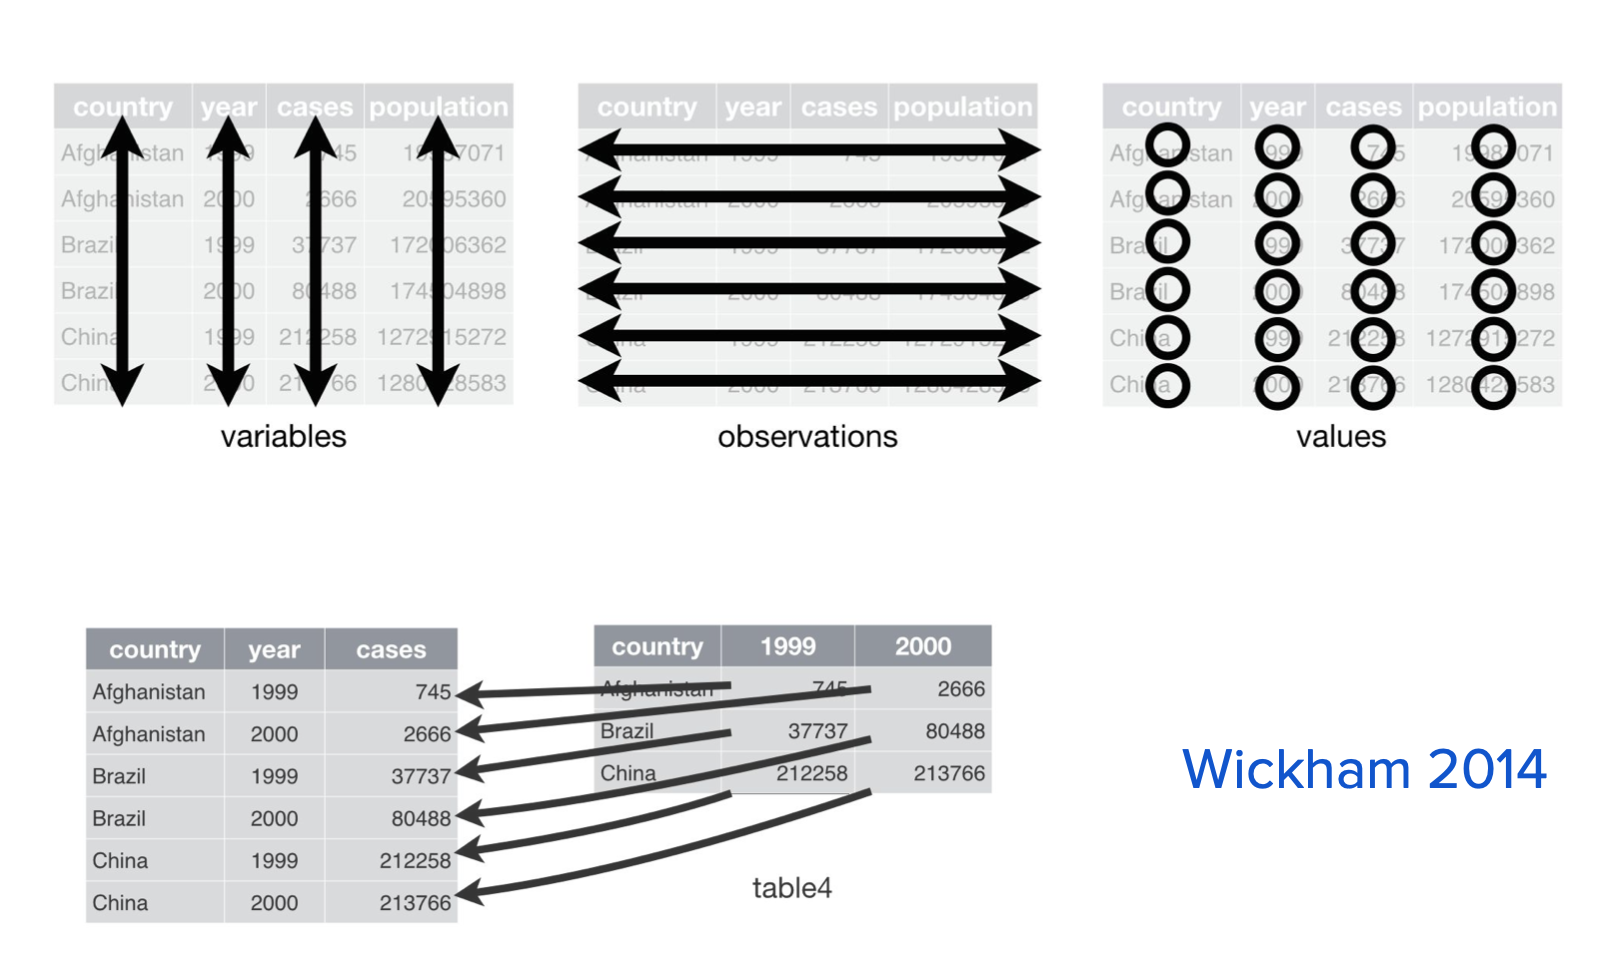
\includegraphics{images/tidy.png}
\caption{Tidy datasets}
\end{figure}

\hypertarget{suxe9ries-temporelles}{%
\subsection{Séries temporelles}\label{suxe9ries-temporelles}}

On parle parfois de \textbf{série temporelle} lorsque une base de donnée concerne un même individu statistique à différents instants. On parle dans ce cas là plutôt d'\textbf{observations} que d'individus. En voilà un exemple : la base de données \texttt{beaver1} accessible dans R présentent la température corporelle d'un castor en fonction du temps.

\begin{table}

\caption{\label{tab:unnamed-chunk-4}Extrait de la base de données beaver1}
\centering
\begin{tabular}[t]{r|r|r|r}
\hline
day & time & temp & activ\\
\hline
346 & 840 & 36.33 & 0\\
\hline
346 & 850 & 36.34 & 0\\
\hline
346 & 900 & 36.35 & 0\\
\hline
346 & 910 & 36.42 & 0\\
\hline
346 & 920 & 36.55 & 0\\
\hline
346 & 930 & 36.69 & 0\\
\hline
\end{tabular}
\end{table}

\hypertarget{autres-types-de-bases-de-donnuxe9es}{%
\subsection{Autres types de bases de données}\label{autres-types-de-bases-de-donnuxe9es}}

\begin{itemize}
\tightlist
\item
  Des données qui décrivent différents individus à un moment donné sont parfois qualifiéed de \textbf{données en coupe} (ou \emph{cross-sectional dataset}). Les données du titanic ou de USArrest en sont des exemples.
\item
  Certaines bases de données décrivent un même groupe d'individus statistique de manière répétée dans le temps. On nomme ce genre de données des \textbf{données de panel} (exemple : enquête Emploi en continu).
\end{itemize}

\hypertarget{variables}{%
\section{Variables}\label{variables}}

\hypertarget{duxe9finition}{%
\subsection{Définition}\label{duxe9finition}}

Les variables sont les éléments qui permettent de décrire les individus présents dans le base de données. Lorsque les données sont issues d'un questionnaire, chaque question correspond en général à une variable.

Exemple :

\begin{itemize}
\tightlist
\item
  le sexe
\item
  la catégorie socioprofessionnelle
\item
  le niveau de diplôme
\item
  le revenu
\end{itemize}

On appelle \textbf{modalités} les différentes valeurs que peuvent prendre une variable.

\begin{figure}
\centering
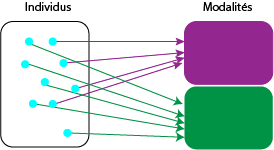
\includegraphics{images/modalites.png}
\caption{Les variables associent les individus à leur modalités}
\end{figure}

\hypertarget{variables-qualitatives-et-variables-quantitatives}{%
\subsection{Variables qualitatives et variables quantitatives}\label{variables-qualitatives-et-variables-quantitatives}}

On distingue les variables en fonction des opérations statistiques qu'on peut effectuer à partir de leurs modalités. Les deux grandes catégories de variables sont les \textbf{variables quantitatives}, dont les modalités sont des nombres, et les \textbf{variables qualitatives}, qui sont les autres.

\hypertarget{variables-qualitatives}{%
\subsection{Variables qualitatives}\label{variables-qualitatives}}

Parmi les variables qualitatives, on distingue encore :

\begin{itemize}
\tightlist
\item
  Les variables \textbf{qualitatives ordinales}, qui sont celles pour lesquelles ont peut ordonner les modalités (exemple : niveau de diplôme)
\item
  Les variables \textbf{qualitatives nominales} dont les modalités ne sont pas hiérarchisables (exemple : sexe, catégorie socioprofesionnelle)
\end{itemize}

\hypertarget{variables-quantitatives}{%
\subsection{Variables quantitatives}\label{variables-quantitatives}}

Les modalités des variables quantitatives (ou numériques) sont des nombres qui ont une signification (par exemple, le code postal n'est pas une variable quantitative). Parmi elles, on distingue :

\begin{itemize}
\tightlist
\item
  Les variables \textbf{continues}, qui peuvent prendre toutes les valeurs réelles dans un intervalle donné
\item
  Les variables \textbf{discrètes}, qui ne peuvent prendre qu'un certain nombre de valeurs
\end{itemize}

\textbf{Pourquoi toutes ces catégories ?} À ces différents types de variables, on associe différentes méthodes statistiques. Il est donc important de comprendre et mémoriser ces définitions, car lorsque vous souhaiterez étudier une variable, la première chose à faire sera d'identifier son type pour ensuite utiliser les méthodes statistiques appropriées.

\hypertarget{mesures-de-tendance-centrale}{%
\section{Mesures de tendance centrale}\label{mesures-de-tendance-centrale}}

Ce sont des manières de résumer l'information contenue dans une variable. En fonction du type de variable, il existe plusieurs indicateurs.

\begin{itemize}
\tightlist
\item
  La \textbf{moyenne} : lorsqu'on parle de moyenne, on fait généralement référence à la moyenne arithmétique d'un ensemble de valeurs numériques (par opposition à la moyenne géométrique ou harmonique). C'est une mesure très utilisée car elle fournit un premier résumé de la distribution statistique. Elle existe uniquement pour les \textbf{variables quantitatives}.
\end{itemize}

\[ \bar{X} = \frac{1}{N}\sum_{i}^{N}{x_i} \]

\begin{itemize}
\item
  La \textbf{médiane} est la modalité d'une variable qui permet de séparer la population en deux parts égales. C'est-à-dire que 50\% des individus auront une modalité supérieure ou égale à la médiane, et 50\% une modalité inférieure ou égale à la médiane.
\item
  Les \textbf{quantiles} sont une généralisation de la médiane : si vous voulez diviser votre population en groupe de 10\%, vous pouvez utiliser les \textbf{déciles}. On appelle la médiane le \textbf{quantile d'ordre 2}, tandis que les déciles sont les \textbf{quantiles d'ordre 10}. Les quantiles les plus utilisés sont la médiane, les quartiles, les déciles et les centiles.
\item
  Les quantiles n'existent que pour les variables dont les modalités peuvent être hiérarchisées : toutes les variables quantitatives et les variables qualitatives ordinales.
\item
  Le \textbf{mode} indique la modalité la plus fréquente d'une variable. Par exemple, la plupart des passagers du Titanic sont décédés dans le naufrage, donc le mode de la variable ``Survived'' est 0.
\end{itemize}

Le mode existe pour tous les types de variables.

\hypertarget{statistique-descriptive-univariuxe9e}{%
\chapter{Statistique descriptive univariée}\label{statistique-descriptive-univariuxe9e}}

Le cours précédent était consacré à vous présenter différents types de variables. Celui de cette semaine présente les premiers éléments de \textbf{statistique descriptive univariée}, les outils permettant la description d'une unique variable. Ces outils dépendent de la nature de la variable étudiée.

\hypertarget{variables-qualitatives-1}{%
\section{Variables qualitatives}\label{variables-qualitatives-1}}

\hypertarget{tris-uxe0-plat}{%
\subsection{Tris à plat}\label{tris-uxe0-plat}}

Pour décrire ce genre de variable, le principal traitement statistique est de compter le nombre d'individus correspondant à chaque modalité de la variable. C'est ce qu'on appelle un \textbf{tri à plat} (par opposition aux tris croisés qui font intervenir plusieurs variables). Un exemple issu des données du titanic @ref(bases-de-données).

\begin{table}
\centering
\begin{tabular}{r|r|r}
\hline
n & \% & val\%\\
\hline
216 & 24.2 & 24.2\\
\hline
184 & 20.7 & 20.7\\
\hline
491 & 55.1 & 55.1\\
\hline
\end{tabular}
\end{table}

\hypertarget{variables-qualitatives-ordinales}{%
\subsection{Variables qualitatives ordinales}\label{variables-qualitatives-ordinales}}

Pour ce genre de variables, on peut ajouter au tri à plat le ``pourcentage cumulé''.

\begin{table}
\centering
\resizebox{\linewidth}{!}{
\begin{tabular}{l|r|r|r|r|r}
\hline
  & n & \% & val\% & \%cum & val\%cum\\
\hline
N'a jamais fait d'etudes & 39 & 2.0 & 2.1 & 2.0 & 2.1\\
\hline
A arrete ses etudes, avant la derniere annee d'etudes primaires & 86 & 4.3 & 4.6 & 6.2 & 6.6\\
\hline
Derniere annee d'etudes primaires & 341 & 17.0 & 18.1 & 23.3 & 24.7\\
\hline
1er cycle & 204 & 10.2 & 10.8 & 33.5 & 35.5\\
\hline
2eme cycle & 183 & 9.2 & 9.7 & 42.6 & 45.2\\
\hline
Enseignement technique ou professionnel court & 463 & 23.2 & 24.5 & 65.8 & 69.7\\
\hline
Enseignement technique ou professionnel long & 131 & 6.6 & 6.9 & 72.4 & 76.6\\
\hline
Enseignement superieur y compris technique superieur & 441 & 22.0 & 23.4 & 94.4 & 100.0\\
\hline
NA & 112 & 5.6 & NA & 100.0 & NA\\
\hline
\end{tabular}}
\end{table}

\hypertarget{repruxe9sentation-graphique}{%
\subsection{Représentation graphique}\label{repruxe9sentation-graphique}}

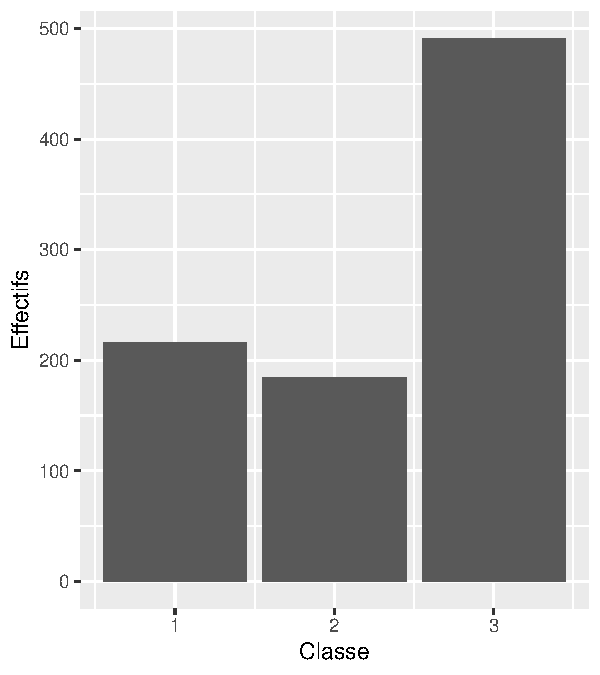
\includegraphics{_main_files/figure-latex/unnamed-chunk-7-1.pdf}

\hypertarget{mesures-de-dispersion}{%
\section{Mesures de dispersion}\label{mesures-de-dispersion}}

\hypertarget{measures-of-dispersion}{%
\subsection{Measures of dispersion}\label{measures-of-dispersion}}

La semaine dernière, je vous ai présenté quelques \textbf{mesures de tendance centrale}. Elles donnent des renseignements importants pour décrire une variable, mais n'en résument qu'une dimension. Deux séries statistiques peuvent avoir la même moyenne tout en étant très différentes.

Comparez par exemple ces deux séries de chiffres, qui représentent des profits (fictifs) en dollars de deux agriculteurs de deux régions A et B :

\begin{itemize}
\tightlist
\item
  A: 14, 16, 18, 20, and 22
\item
  B: 2, 8, 18, 29, and 33
\end{itemize}

\hypertarget{mesures-de-dispersion-1}{%
\subsection{Mesures de dispersion}\label{mesures-de-dispersion-1}}

La somme de ces deux série est la même, 90 dollars, mais il apparaît rapidement que l'une des séries est beaucoup plus \textbf{dispersée} que l'autre, c'est-à-dire que les écarts par rapport à la moyenne sont en général beaucoup plus grands (la série B). Notre vision des risques et des profits liés à l'agriculture dans est informée de cette différence, et nous devrions en inclure des indices dans toute description statistique de cette variable.

Pour faire cela, nous avons besoin de mesures permettant de décrire la disperion des modalités de la variable autour de sa moyenne. Toutes ces mesures n'existent que pour deq \textbf{variables quantitatives}.

\hypertarget{luxe9tendue}{%
\subsection{L'étendue}\label{luxe9tendue}}

C'est la différence entre la plus grande et la plus petite valeur de la série :

\[R = X_{max} - X_{min}\]

C'est une mesure de dispersion assez basique.

\hypertarget{luxe9cart-interquartile}{%
\subsection{L'écart interquartile}\label{luxe9cart-interquartile}}

Plutôt que de calculer la différence entre le maximum et le minimum, on peut calculer la différence entre deux quantiles, des quartiles par exemple (rappel de la définition ?).

\[ Q_d = Q_3 - Q_1 \]

C'est un mesure un peu meilleure que l'étendue, parce que le maximum et le minimum sont des valeurs qui donnent généralement peu d'information sur la distribution en général.

\hypertarget{la-variance}{%
\subsection{La variance}\label{la-variance}}

La variance est égale à la moyenne arithmétique des écarts à la moyenne au carré. C'est une manière de mesurer \textbf{un écart moyen à la moyenne}.

\[ s^2 = \frac{1}{n} \sum_{i = 1}^{n} (X_i - X_m)^2 \]

\hypertarget{luxe9cart-type}{%
\subsection{L'écart type}\label{luxe9cart-type}}

\[ \sigma = \sqrt{\frac{1}{n} \sum_{i = 1}^{n} (X_i - X_m)^2} \]

L'écart-type est la mesure de dispersion la plus utile et la plus fréquente. Elle est meilleure que la variance car elle se mesure dans la même unité que la variable en question (tandis que la variance se mesure dans l'unité de la variable au carré). Par exemple, on peut dire que dans la région A, la moyenne des revenus agricoles est de 18 dollars, avec un écart-type de 2,8 dollars.

\hypertarget{la-moyenne-ponduxe9ruxe9e-rajout-uxe0-la-liste-des-mesures-de-tendance-centrale-de-la-semaine-derniuxe8re}{%
\subsection{La moyenne pondérée (rajout à la liste des mesures de tendance centrale de la semaine dernière)}\label{la-moyenne-ponduxe9ruxe9e-rajout-uxe0-la-liste-des-mesures-de-tendance-centrale-de-la-semaine-derniuxe8re}}

\begin{table}
\centering
\begin{tabular}{r|r}
\hline
Pclass & Age\_m\\
\hline
1 & NA\\
\hline
2 & NA\\
\hline
3 & NA\\
\hline
\end{tabular}
\end{table}

\[ Age_m = \frac{1}{n} \sum_{j} n_j*Age_j \] où \(Age_j\) est la moyenne de la \(j^{ième}\) catégorie.

\hypertarget{distributions}{%
\section{Distributions}\label{distributions}}

\hypertarget{histogrammes}{%
\subsection{Histogrammes}\label{histogrammes}}

Les histogrammes sont l'équivalent des diagrammes en barres pour les variables quantitatives. Chaque barre (ou rectangle) qui compose l'histogramme a une aire qui est proportionnelle au nombre d'observation dont les valeurs sont dans l'intervalle sur lequel s'étend le rectangle.

\begin{verbatim}
## `stat_bin()` using `bins = 30`. Pick better value with `binwidth`.
\end{verbatim}

\begin{verbatim}
## Warning: Removed 177 rows containing non-finite values (stat_bin).
\end{verbatim}

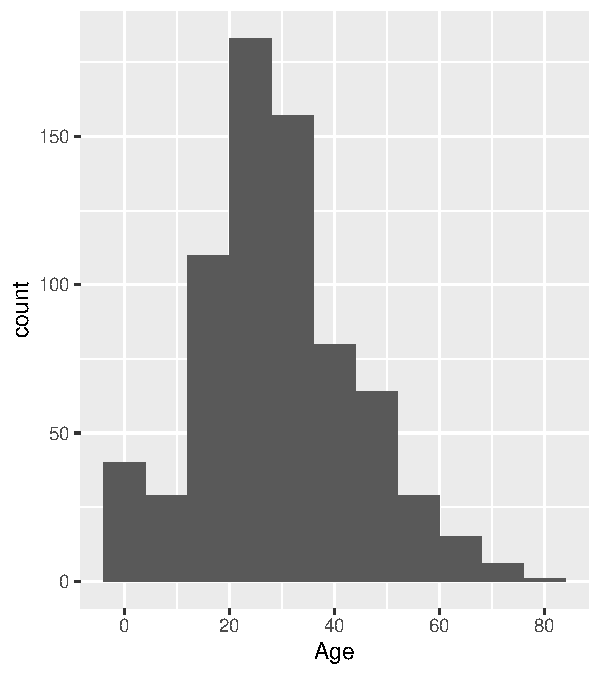
\includegraphics{_main_files/figure-latex/unnamed-chunk-9-1.pdf}

\hypertarget{histogrammes-1}{%
\subsection{Histogrammes}\label{histogrammes-1}}

Comme il s'agit de variables quantitatives, on peut choisir le nombre de rectangles comme on le souhaite. Ici, on représente la même variable avec moins de rectangles.

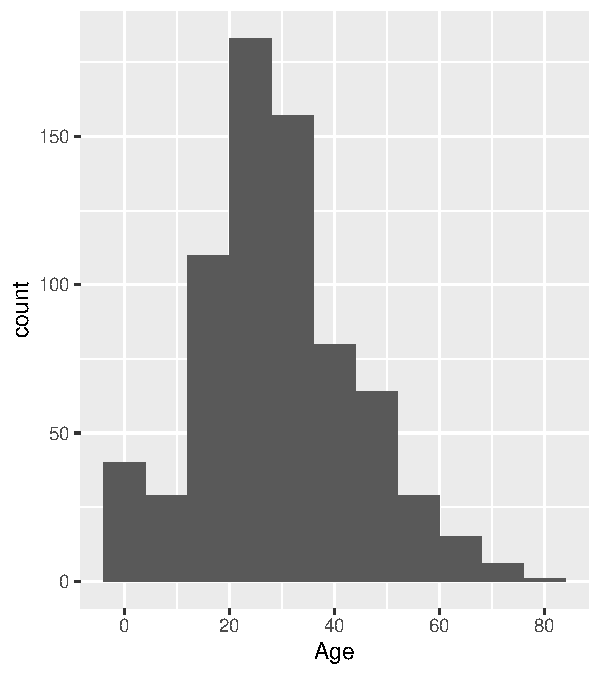
\includegraphics{_main_files/figure-latex/unnamed-chunk-10-1.pdf}

\hypertarget{histogrammes-2}{%
\subsection{Histogrammes}\label{histogrammes-2}}

Ici avec un plus grand nombre de rectangle (largeur = 1 an)

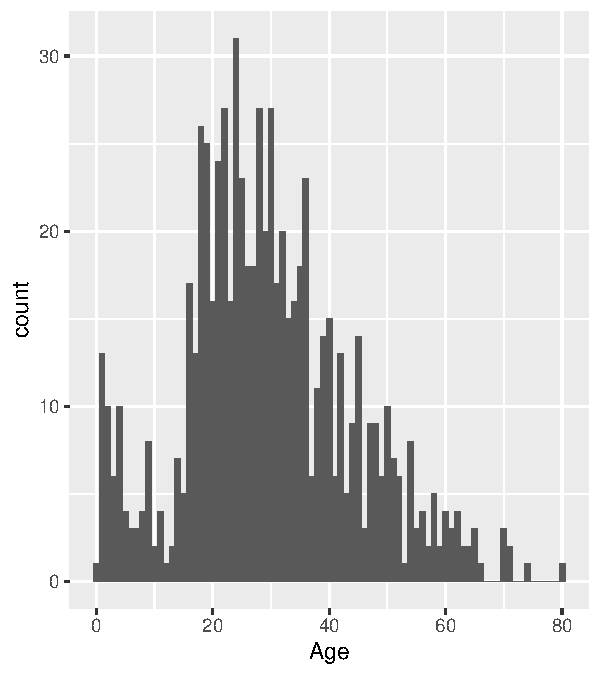
\includegraphics{_main_files/figure-latex/unnamed-chunk-11-1.pdf}

\hypertarget{polygone-de-fruxe9quence}{%
\subsection{Polygone de fréquence}\label{polygone-de-fruxe9quence}}

On peut tracer une ligne qui passe au milieu de chacun des segments supérieurs des rectangles qui composent l'histogramme, on appelle ce graph un polygone de fréquence.

\begin{figure}
\centering
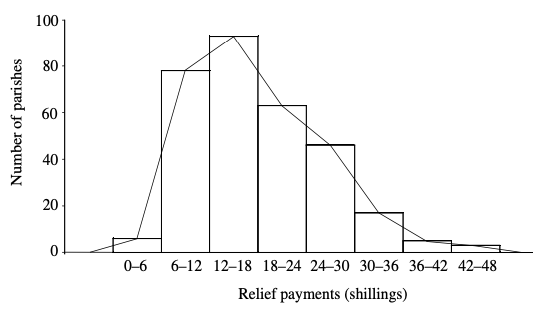
\includegraphics[width=3.125in,height=\textheight]{images/frequencypol.png}
\caption{\emph{Per capita} relief payments in 311 parishes in 1831 (Fenstein \& Thomas, p.~41)}
\end{figure}

\hypertarget{densituxe9}{%
\subsection{Densité}\label{densituxe9}}

La forme de ce polygone peut être être ``lissée'' à l'aide de techniques mathématiques, pour donner ce qu'on appelle une courbe de densité. Elle donne une idée de la forme du polygon de fréquence si l'on avait un très grand nombre d'individu dans notre échantillon.

\begin{figure}
\centering
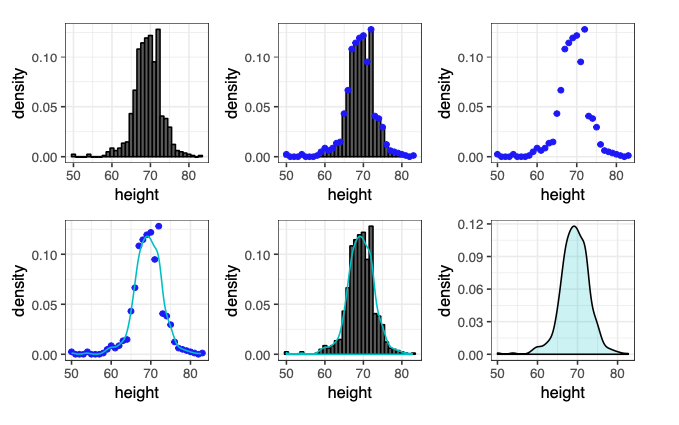
\includegraphics{images/density.png}
\caption{D'un histogramme à une densité de probabilité}
\end{figure}

\hypertarget{distributions-1}{%
\subsection{Distributions}\label{distributions-1}}

Ces représentations graphiques sont un bon moyen de visualiser la \textbf{forme} de la distribution d'une variable quantitative continue, et spécifiquement de la manière dont les données sont réparties autour de leur valeur ``centrale''. Elles peuvent être réparties symétriquement ou bien de manière asymétrique.

\hypertarget{distributions-2}{%
\subsection{Distributions}\label{distributions-2}}

\begin{figure}
\centering
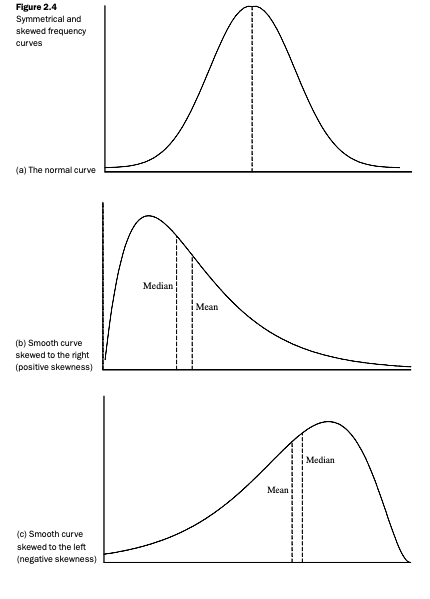
\includegraphics{images/skewed.png}
\caption{Symmetrical and skewed distributions (Fenstein \& Thomas, p.~54)}
\end{figure}

\hypertarget{mesure-de-lasymuxe9trie-skewness}{%
\subsection{\texorpdfstring{Mesure de l'asymétrie (\emph{skewness})}{Mesure de l'asymétrie (skewness)}}\label{mesure-de-lasymuxe9trie-skewness}}

\begin{itemize}
\tightlist
\item
  Elles doivent être indépendantes de l'unité de mesure
\item
  Et elle doivent être nulles lorsque la distribution est symétrique.
\end{itemize}

Un exemple de coefficient d'asymétrie est le suivant, mais il en existe d'autres :

\[ Skewness = \frac{3*(Mean - Median)}{\sigma} \]

\hypertarget{la-loi-normale}{%
\subsection{La loi normale}\label{la-loi-normale}}

C'est une distribution théorique qui correspondant un nombre de cas infini. Bien que théorique, c'est une distribution très utilisée comme approximation de distributions réelles.

\hypertarget{la-loi-normale-1}{%
\subsection{La loi normale}\label{la-loi-normale-1}}

La coubre de la loi normale implique deux constantes : la moyenne \(X_m\) et l'écart type \(\sigma\). L'équation donne la valeur de Y (la hauteur de la courbe, qui apparaît sur l'axe des ordonnées) pour tout valeru de X (mesuré sur l'axe des abscisses).

\[ Y = \frac{1}{ \sigma \sqrt{2\pi}} exp(- \frac{(X - X_m)^2}{2*\sigma^2})\]

\hypertarget{dispersion-de-la-loi-normale}{%
\subsection{Dispersion de la loi normale}\label{dispersion-de-la-loi-normale}}

Une propriété importante de la loi normale est que, quelque soit sa moyenne et son écart-type, il y a toujours une même proportion d'observation qui seront distribués à une certaine distance de la moyenne, mesurée en nombre d'écarts-type.

Par exemple :

\begin{itemize}
\tightlist
\item
  \textbf{90\% des observations} sont situés à moins de \textbf{1,645 écarts-type} autour de la moyenne, laissant 5\% de chaque côté.
\item
  \textbf{95\% des observations} sont situés à moins de \textbf{1,96 écarts-type} autour de la moyenne, laissant 2,5\% de chaque côté.
\item
  \textbf{99\% des observations} sont situés à moins de \textbf{2,58 écarts-type} autour de la moyenne, laissant 0,5\% de chaque côté.
\end{itemize}

\hypertarget{dispersion-de-la-loi-normale-1}{%
\subsection{Dispersion de la loi normale}\label{dispersion-de-la-loi-normale-1}}

\begin{figure}
\centering
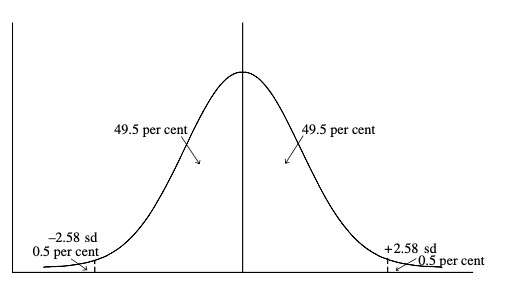
\includegraphics{images/normal.png}
\caption{Aire sous la courbe}
\end{figure}

\hypertarget{ruxe9fuxe9rences}{%
\chapter*{Références}\label{ruxe9fuxe9rences}}
\addcontentsline{toc}{chapter}{Références}

  \bibliography{book.bib}

\end{document}
